% ----------------------------------------------------------
% Revisão bibliográfica
% ----------------------------------------------------------
\chapter{Revisão da literatura}
\label{chp:revisão}

Os principais aspectos relacionados à coleta de evidências para análise forense em nuvem são: coleta, transporte, armazenamento, garantia da cadeia de custódia e reprodutibilidade do processo de coleta. 
%
Nesta seção são discutidas propostas encontradas na literatura que envolvem tais aspectos, com o objetivo de dar ao leitor uma visão geral do estado da arte na área.

\marcos{Separe em seções essa discussão: isso facilita muito a leitura. Também precisa traduzir as figuras: seu texto está em português, então não faz sentido suas figuras estarem em inglês. Isso vale para qualquer figura, tabela, etc., mesmo se forem de outros trabalhos. Simplesmente diga que foi ``Adaptado de REFERENCIA'' quando for apresentar a figura}

O modelo proposto por \cite{ReichertAutoAcquisition:2015} é um processo de coleta de evidências integrado ao \textit{hypervisor} e disparado por algum sistema de detecção de intrusão. 
%
A partir do momento em que uma ameaça é detectada, o modelo tira instantâneos das máquinas virtuais comprometidas. O modelo toma cuidado para excluir informações de clientes não relacionados a investigação e armazena o restante em local seguro, tudo de forma automatizada.
%
O autor não descreve os detalhes do armazenamento mas diz que é ``forensicamente aceitável''.
%
O modelo faz uso de GRR ( \textit{Google Rapid Response} -- Resposta Rápida Google ) para agregar e analisar as evidências coletadas. 
%
O modelo possui um motor de regras que se baseia em um conjunto de descrições de ameaças conhecidas armazenadas em banco para, caso alguma evidência coletada coincida com ameaças armazenadas, ele alerta um usuário humano para uma avaliação mais detalhada.
%
O intervalo de tempo em que os instantâneos de memória são gerados é configurável e são todos armazenados em persistência.
%
Este modelo tem como principal vantagem a automação do processo de coleta que dispensa intervenção humana. 
%
A figura \ref{fig:ReichertAutoAcquisitionModel} mostra o desenho da arquitetura proposta pelo autor.

\begin{figure}[htb!]
\footnotesize
\caption{\textit{Automated Forensics Data Acquisition Model}}
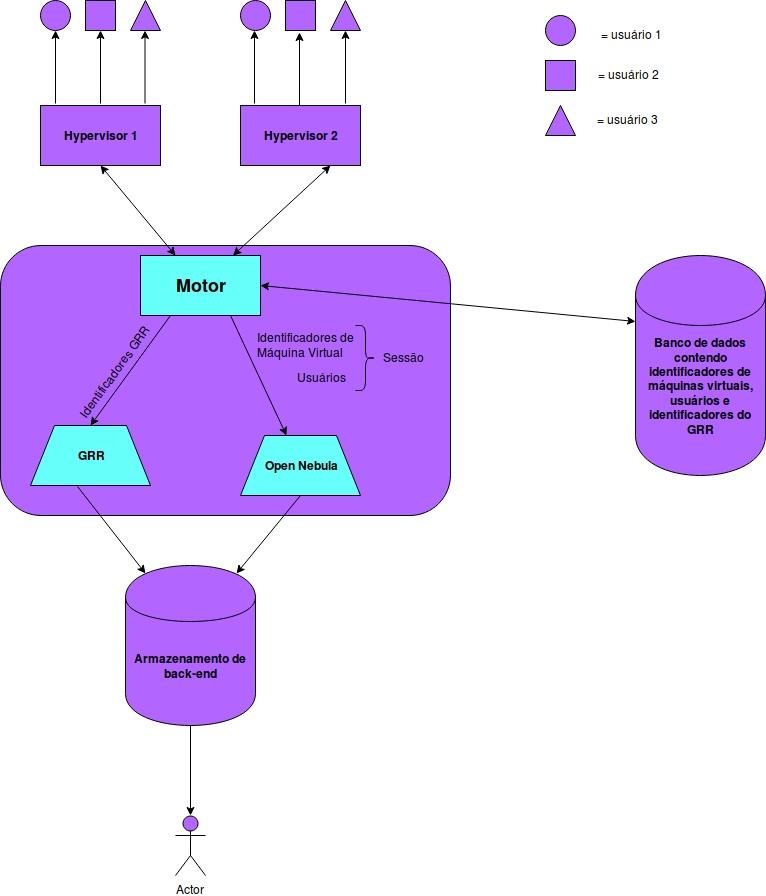
\includegraphics[scale=0.50]{ReichertAutoAcquisitionModel.png}
\centering
\label{fig:ReichertAutoAcquisitionModel}
\begin{center}
Adaptado de \cite{ReichertAutoAcquisition:2015} 
\end{center}
\end{figure}

A proposta de \cite{PoiselVMI:2013} é baseada na técnica de VMI ( \textit{Virtual Machine Introspection} -- Introspecção em Máquina Virtual ) para coleta de memória volátil. 
%
Esta técnica se apoia na necessidade do VMM ( \textit{Virtual Machine Manager} -- Gerenciador de Máquinas Virtuais ) em mapear recursos físicos da máquina hospedeira a recursos alocados à máquina virtual cliente.
%
Este mapeamento é usado para permitir que a memória volátil copiada da máquina virtual seja reconstruída em uma máquina física para realização da análise.
%
A proposta utiliza de coleta contínua dos instantâneos de memória durante o funcionamento do sistema sem distinção do que aconteceu antes ou depois do fato de interesse, e todos os instantâneos de memória são armazenados para posterior análise.
%
Para eliminar a chance de inconsistências no instantâneo de memória volátil, a máquina virtual tem sua execução suspensa durante o processo de extração.
%
Uma desvantagem da técnica de VMI mencionado pelo próprio autor é a necessidade de tradução de endereços de memória da máquina virtual em endereços de memória da máquina física hospedeira.
%
Esta tradução depende de conhecimento do que está sendo executado na máquina virtual, logo uma solução baseada em VMI não é completamente portável sendo necessário adequações para diferentes clientes além de ser computacionalmente custoso.
%

Também na vertente de introspecção de máquina virtual, \cite{Dolan-GavittSemanticGap:2011} propõe o \textit{Virtuoso}, um arcabouço de coleta de informações de processos específicos em uma máquina virtual.
%
O arcabouço funciona em três fases, a primeira realiza um estudo em uma máquina virtual teste do processo que se deseja coletar dados de memória mapeando o conjunto de instruções executado. 
%
A fase dois traduz o conjunto de instruções mapeados na fase um e cria um executável para que o processo seja rodado fora da máquina virtual.
%
A terceira fase usa um ambiente na máquina hospedeira para executar as instruções extraídas na fase dois. Este ambiente consegue acessar os endereços de memória do máquina virtual tornando possível coletar instantâneos de memória do processo em execução.
%
A principal vantagem deste arcabouço é a capacidade de coletar instantâneos de memória de um processo específico.
%
A desvantagem deste método é que sua atuação é após o fato.
%
A figura \ref{fig:Dolan-GavittSemanticGap} mostra um esquema do funcionamento do arcabouço

\begin{figure}[htb!]
\footnotesize
\caption{Virtuoso}
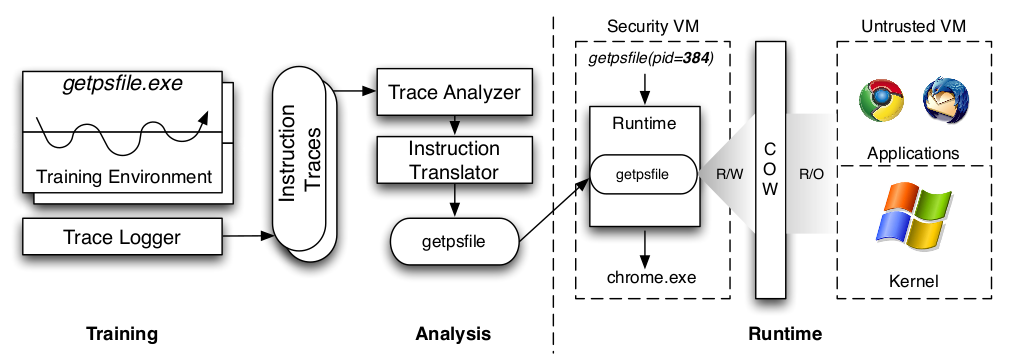
\includegraphics[scale=0.40]{Dolan-GavittSemanticGap.png}
\centering
\label{fig:Dolan-GavittSemanticGap}
\begin{center}
Adaptado de \cite{Dolan-GavittSemanticGap:2011} 
\end{center}
\end{figure}


O arcabouço proposto por \cite{SangLogApproach:2013} é um sistema que funciona em parceria com o provedor de nuvem onde este último envia informações ao arcabouço que os armazena em um local centralizado.
%
O conjunto de informações armazenadas é acordado antecipadamente com o provedor de nuvem e vão desde instantâneos de memória volátil até pacotes trafegados nas interfaces de rede da máquina virtual.
%
O arcabouço coleta informações continuamente e usa cálculo de hash das evidências enviadas pelo provedor de nuvem para garantir que elas não foram alteradas durante o transporte.
%
Assim como as propostas anteriores, esta também não faz distinção do que aconteceu antes ou depois do fato de interesse coletando constantemente informações da máquina virtual.
%
O próprio autor menciona que o arcabouço tem a desvantagem de depender da cooperação do provedor de nuvem. Esta dependência é uma estratégia considerada fraca pela comunidade forense pois a prioridade do CSP ( \textit{Cloud Service Provider} -- Provedor de Serviços de Nuvem ) é o de garantir a disponibilidade do serviço não o de coletar evidências \cite{ClarkeReviewOfChallenges2015}.
%
A figura \ref{fig:SangLogApproach} mostra um esquema do funcionamento da solução focada em um caso específico de log de rede como proposta pelo autor.

\begin{figure}[htb!]
\footnotesize
\caption{\textit{A Log Based Approach Model}}
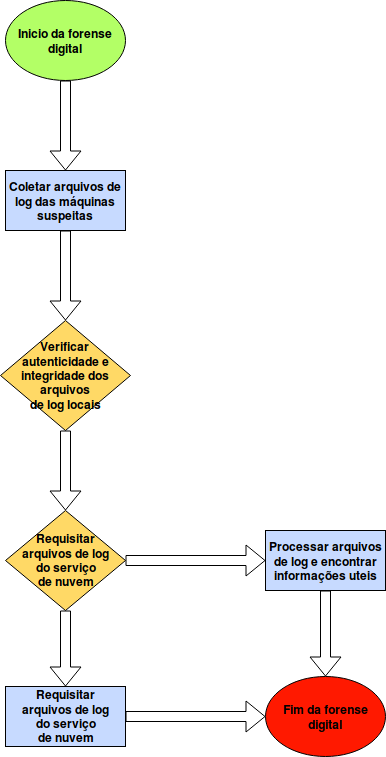
\includegraphics[scale=0.50]{SangLogApproach.png}
\centering
\label{fig:SangLogApproach}
\begin{center}
Adaptado de \cite{SangLogApproach:2013} 
\end{center}
\end{figure}

O trabalho descrito em \cite{DezfouliBackupApproach:2012} é voltada a dispositivos móveis e tem como principal vantagem a preocupação com as limitações de armazenamento do dispositivo.
%
O processo de coleta do instantâneo de memória volátil do dispositivo separa as informações e as armazena por processo ativo, o autor usa esta técnica para melhor gerenciar o espaço que as informações estão ocupando em disco. 
%
Possui inteligência para descartar informações de processos que foram terminados e removidos da memória assim como inteligência para fazer uso ótimo do espaço de armazenamento do dispositivo.
%
O processo de coleta de informações de memória volátil é feita continuamente independente de eventos de interesse como detecção de ameaças.
%
A figura \ref{fig:DezfouliBackupApproach} o autor mostra um esquema macro de como o armazenamento da evidência é gerenciado.

\begin{figure}[htb!]
\footnotesize
\caption{\textit{Backup Approach Model}}
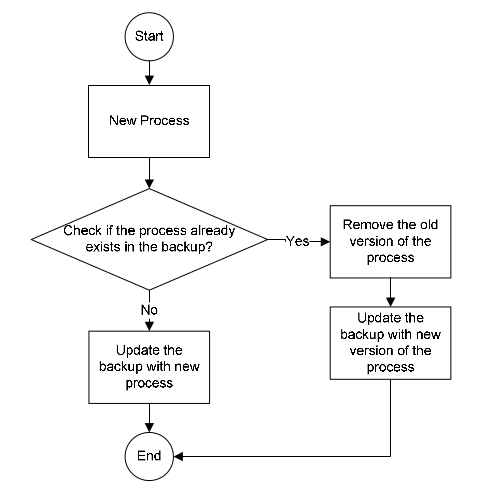
\includegraphics[scale=0.50]{DezfouliBackupApproach.png}
\centering
\label{fig:DezfouliBackupApproach}
\begin{center}
Adaptado de \cite{DezfouliBackupApproach:2012} 
\end{center}
\end{figure}

A ferramenta FROST ( \textit{FoRensic Open Stack Tools} -- Ferramentas Forenses para Arcabouço Open Stack ) proposto por \cite{DykstraFROST:2013} descreve um conjunto de bibliotecas integradas ao arcabouço \textit{Open Stack Framework} de gerenciamento de infra estruturas virtualizadas.
%
Através desta integração, FROST expõe um conjunto de API para serem usadas por aplicações de coleta de evidências forenses que dão acesso a recursos da máquina virtual sendo administrada como disco, logs de trafego de rede e memória volátil.
%
A proposta descreve apenas o arcabouço, deixa a critério do usuário detalhes como periodicidade e tamanho da coleta assim como a forma de transporte da evidência e onde ela será armazenada.
%
De todas as propostas descritas neste capítulo esta é a única que demonstra preocupação com adequação a questões legais e padrões já estabelecidos na industria forense.
%
O autor declara que FROST segue as práticas definidas no SWGDE ( \textit{Scientific Working Group on Digital Evidence} -- Grupo de Pesquisa Scientífica Em Evidência Digital ) e do Manual de Busca em Apreensão do Departamento de Justiça Norte-Americano.
%
A figura \ref{fig:DykstraFROST} o autor mostra um esquema macro da integração entre FROST e o arcabouço \textit{Open Stack}

\begin{figure}[htb!]
\footnotesize
\caption{\textit{FoRensic Open Stack Tools}}
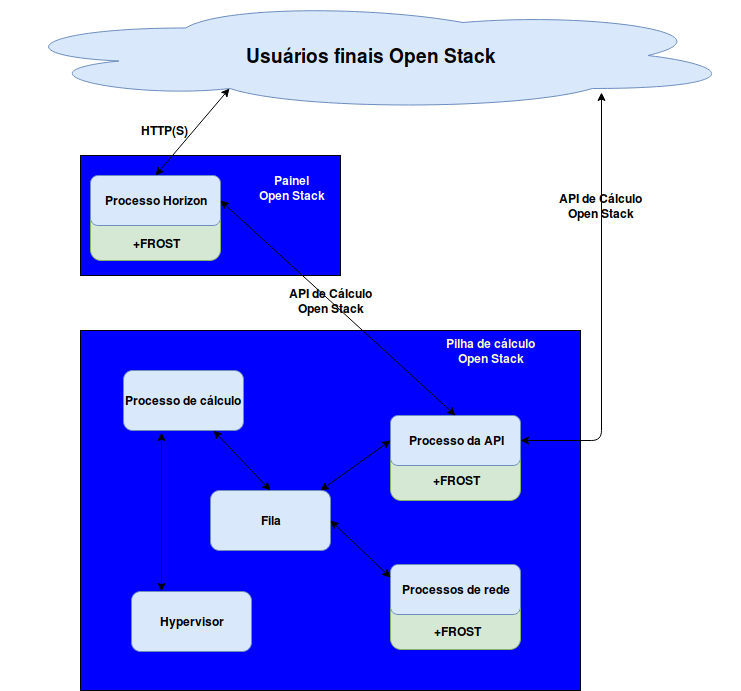
\includegraphics[scale=0.50]{DykstraFROST.png}
\centering
\label{fig:DykstraFROST}
\begin{center}
Adaptado de \cite{DykstraFROST:2013} 
\end{center}
\end{figure}
%

O trabalho descrito em \cite{GeorgeDF2CE:2012} está focado em monitoração de rede e opera em uma arquitetura FaaS ( \textit{Forense as a Service} -- Forense Como Serviço ). 
%
O autor propõe um conjunto de ferramentas que tem capacidade de realizar auto descoberta das interfaces sob monitoração, coletar evidências de tais máquinas e armazená-las.
%
O processo de auto descoberta e associação das evidências com usuários de rede é realizado por um motor baseado em ontologias armazenadas em um banco de dados próprio.
%
Esta proposta foca apenas no processo de coleta. A descrição do armazenamento e transporte é superficial.
%
Na figura \ref{fig:GeorgeDF2CE} mostra o desenho da arquitetura proposta pelo autor.

\begin{figure}[htb!]
\footnotesize
\caption{\textit{Digital Forensic Framework for Cloud Environment}}
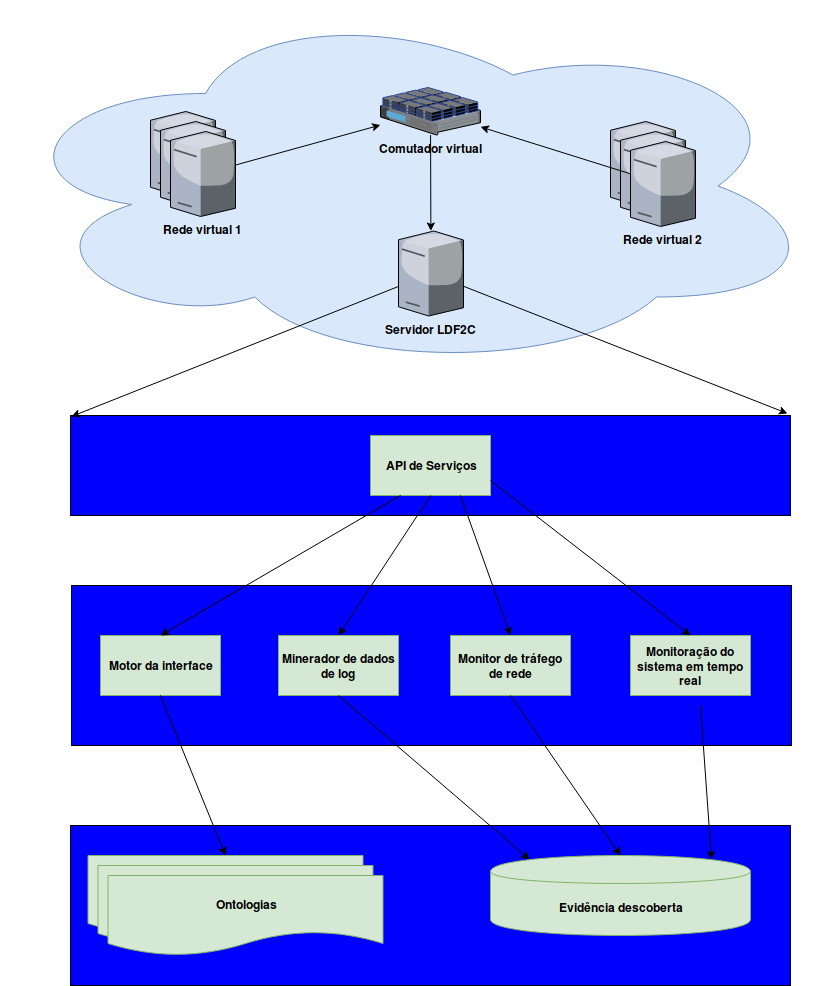
\includegraphics[scale=0.50]{GeorgeDF2CE.png}
\centering
\label{fig:GeorgeDF2CE}
\begin{center}
Adaptado de \cite{GeorgeDF2CE:2012} 
\end{center}
\end{figure}

Na mesma vertente de forense como serviço, \cite{FaaSIndexedSearch:2012} ataca o problema de grande volume de dados coletados propondo serviço de coleta e indexação de evidências.
%
O serviço espera receber dados da execução do comando unix DD \cite{UnixManPagesDD} nas máquinas alvo onde, apoiado em processos ETL ( \textit{Extract, Transform and Load} -- Extrair, Transformar e Carregar ) e MapReduce \cite{WikipediaMapReduce}, os dados serão disponibilizados para consulta pelos investigadores.
%
A coleta ocorre continuamente a intervalos de tempo configuráveis.
%
O autor não descreve onde os dados serão armazenados e quem será responsável pela infraestrutura de armazenamento.
%
O autor também não fala como os dados serão transportados até o armazenamento e como ele garante que estes não foram alteramos no processo.
%
A figura \ref{fig:FaaSIndexedSearch} mostra o desenho da arquitetura do serviço proposta pelo autor

\begin{figure}[htb!]
\footnotesize
\caption{\textit{Digital Forensic as a Service - Indexed Data}}
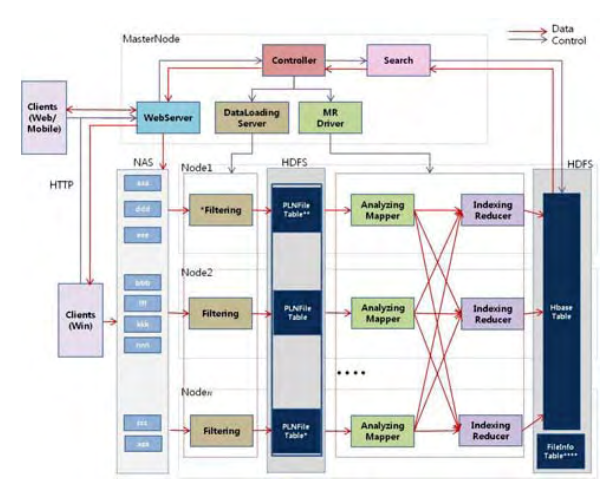
\includegraphics[scale=0.45]{FaaSIndexedSearch.png}
\centering
\label{fig:FaaSIndexedSearch}
\begin{center}
Adaptado de \cite{FaaSIndexedSearch:2012} 
\end{center}
\end{figure}

A seguir os trabalhos mencionados acima são agrupados e avaliados com base nos diferentes aspectos que abordam.

\section{Acessar e coletar as informações de memória das máquinas virtuais em nuvem}
\label{sec:coletadeevidencia}

Diversos trabalhos de análise forense na nuvem se concentram na coleta de dados ``após o fato'', ou seja, após a intrusão ser detectada \cite{ReichertAutoAcquisition:2015,PoiselVMI:2013,DykstraFROST:2013,GeorgeDF2CE:2012,SangLogApproach:2013}. 
%
Os processos de coleta descritos nesses trabalhos podem ser iniciados de forma manual ou automaticamente, via integração com um mecanismo de detecção de intrusão. 
%
No caso específico de memória volátil, tal forma de coleta não consegue descrever como era a memória antes da intrusão, pois o processo só é acionado depois da detecção do ataque. 
%
%A capacidade de saber como era a memória antes do fato é descrita por \cite{Case_Memory_Forensics:2014} como necessária para viabilizar a abordagem de coletar o suficiente para realizar a investigação pois permite comparar dois instantâneos de memória e minimizar o volume coletado antes do fato. 
Tal limitação pode trazer prejuízos à investigação, dado que algumas análises dependem exatamente da capacidade de se comparar dois momentos da memória \cite{CaseMemoryForensics:2014}. 
%
Entre os trabalhos estudados, a única proposta encontrada que leva tal necessidade em consideração é \cite{DezfouliBackupApproach:2012}, que propõe que o dado seja armazenado no próprio equipamento sob análise.
%
%Infelizmente, entretanto, essa abordagem não é aplicável ao cenário em nuvem, pois leva a perda de informações importantes caso a máquina virtual seja despejada e seus recursos liberados.
Infelizmente, entretanto, a aplicação de tal abordagem no cenário em nuvem é pouco viável, pois pode levar à perda de informações importantes caso a máquina virtual ou contêiner seja desativada, tendo seus recursos liberados.
%

%Ainda na coleta de informações, os autores \cite{Reichert_Auto_acquisition:2015} e \cite{George_DF2CE:2012} sugerem a abordagem de forense ao vivo onde os dados são constantemente coletados sem distinção do antes ou depois do fato. 
Existem ainda trabalhos voltados à coleta de informações durante a execução do sistema, nos quais os dados são constantemente coletados sem distinção do que aconteceu antes ou depois do fato de interesse.
%
Esse é o caso de trabalhos como \cite{PoiselVMI:2013,DykstraFROST:2013,SangLogApproach:2013,Dolan-GavittSemanticGap:2011}, que adotam a estratégia de isolar e parar a máquina virtual para em seguida realizar o processo de coleta. 
%
%Nas duas estratégias citadas anteriormente, o problema do grande volume de informações coletadas não é abordado pelo autores nem o cenário onde é necessário coletar evidências de uma máquina virtual que já foi despejada do pool e os recursos liberados. 
Embora interessantes, as abordagens descritas nesses trabalhos podem levar a um elevado volume de dados coletados, além de também não tratarem o cenário em que é necessário coletar evidências quando os recursos virtuais contendo tais informações são liberados.


\section{Capacidade de reproduzir o processo e obter os mesmos resultados}
\label{sec:reprodutibilidade}

Se, durante uma análise forense, analistas diferentes obtêm resultados distintos ao executar o mesmo procedimento de coleta, a evidência gerada não tem credibilidade, inviabilizando seu uso em um processo legal. 
%
Por essa razão, a reprodutibilidade do processo de coleta é uma parte importante da geração de evidências para análise forense.
%
Infelizmente, entretanto, nenhuma das propostas encontradas na literatura atualmente permite tal reprodutibilidade em cenários de nuvem em que máquinas virtuais ou contêineres são desativados e seus recursos físicos liberados: todas elas dependem da existência do recurso virtual para a repetição do processo de coleta.

\section{Não violar privacidade ou jurisdição das partes não envolvidas na investigação}
\label{sec:legais}

Em um ambiente de nuvem pública, remover o \textit{hardware} para análise posterior pode levar à violação de privacidade de usuários, uma vez que o multi-inquilinato desse cenário faz com que uma mesma máquina física guarde informações de diversos clientes, alguns dos quais podem não estar envolvidos na investigação em curso.
%
Diversos trabalhos na literatura tratam esse problema adequadamente, por meio das duas estratégias principais: a primeira, adotada em \cite{ReichertAutoAcquisition:2015,GeorgeDF2CE:2012,PoiselVMI:2013,DykstraFROST:2013,FaaSIndexedSearch:2012}, consiste em coletar dados pertinentes à investigação e armazená-los fora da nuvem; a segunda, empregada em \cite{SangLogApproach:2013} e que constitui um caso específico de \cite{GeorgeDF2CE:2012}, depende da cooperação do provedor de serviços de nuvem para conseguir as informações necessárias à investigação. 
%
Depender do provedor de serviços de nuvem é uma estratégia pouco recomendada, entretanto, pois (1) o volume de dados de usuários pode forçar os provedores a limitar o tamanho dos \textit{logs} armazenados, e (2) caso ocorra uma indisponibilidade causada por um ataque, o objetivo do provedor será o de restabelecer o serviço, não necessariamente o de preservar evidências\cite{ClarkeReviewOfChallenges2015}. 


\section{Garantir a cadeia de custódia da evidência}
\label{sec:cadeiadecustodia}

Dentre os trabalhos analisados, apenas \cite{SangLogApproach:2013} aborda a questão da garantia da cadeia de custódia. 
%
Especificamente, o trabalho emprega \textit{hashes} para verificar a integridade da evidência, permitindo a detecção de alterações na mesma, embora não explique os mecanismos que poderiam ser utilizados para impedir acesso não autorizado (e, assim, potencial alteração) aos próprios hashes. 
%
As propostas dos outros autores concentram-se apenas no aspecto técnico da coleta, sem discutir claramente garantia de custódia mas apenas mencionando que as evidências devem ser coletadas de forma forensicamente aceitável.

\section{Resumo}

A Tabela \ref{tab:related-work} mostra um comparativo das soluções estudadas, considerando os aspectos discutidos nesta seção, posicionando as contribuições da proposta apresentada neste trabalho.

\begin{table}[htb!]
\footnotesize
\renewcommand{\arraystretch}{1.4}
\renewcommand{\tabcolsep}{0.5mm}
\centering
\caption{Comparativo de soluções de coleta de informações de memória de máquinas em nuvem para análise forense}
\label{tab:related-work}
\begin{tabular}{p{5.3cm}|L|L|L|L|L|L|L|L|L|}
\textbf{}						& \rot{\fancyname~(esta proposta)} 			& \rot{\cite{GeorgeDF2CE:2012}} 
							& \rot{\cite{PoiselVMI:2013}} 				& \rot{\cite{DykstraFROST:2013}}
							& \rot{\cite{FaaSIndexedSearch:2012}} 			& \rot{\cite{ReichertAutoAcquisition:2015}}	
							& \rot{\cite{SangLogApproach:2013}} 			& \rot{\cite{Dolan-GavittSemanticGap:2011}} 
							& \rot{\cite{DezfouliBackupApproach:2012}} 				
\\ \hline
\textbf{Coleta é contínua?}				& \cfig	& \xfig & \xfig & \xfig & \cfig & \xfig & \cfig & \xfig & \cfig  \\
\textbf{Reproduz o processo sem a VM?} 			& \cfig	& \xfig & \xfig & \xfig & \xfig & \xfig & \xfig & \xfig & \xfig  \\
\textbf{Garante cadeia de custódia?}			& \cfig	& \xfig & \xfig & \xfig & \xfig & \cfig & \cfig & \xfig & \xfig  \\
\textbf{Preserva jurisdição e privacidade?} 		& \cfig	& \cfig	& \cfig	& \cfig	& \cfig	& \cfig	& \cfig	& \cfig	& \cfig	 \\
\end{tabular}
\end{table}
